\documentclass{article}
\usepackage{iclr2026_conference,times}
\usepackage{amsmath,amssymb,booktabs,graphicx,url}
\usepackage[utf8]{inputenc}
\usepackage[T1]{fontenc}
\usepackage{hyperref}
\iclrfinalcopy

\title{Embodied Prompting\\for Nonverbal Robot Tasks}

\author{Anonymous Authors}

\begin{document}
\maketitle

\begin{abstract}
Robot prompting is usually treated as text plus pixels: the user says what to do, an image supplies context, and a model chooses an action. Many practical robot instructions are not spoken or written. A person points, holds an object out, taps a fixture, blocks a motion with an open palm, or demonstrates a short path. We propose embodied prompting: representing nonverbal cues as typed physical state that can bind to objects, affordances, and safety-critical action commitments. The recovery sweep for this paper produced 240 structured related-work rows and narrowed the contribution away from generic multimodal prompting. On 540 synthetic nonverbal instruction cases, text-only prompting reaches 0.165 task accuracy, captioned cues reach 0.819, and an embodied prompt graph reaches 0.978 while reducing unsafe prompt execution from 0.678 to 0.000. A v2 safety-cue binding stress narrows the claim: at a 5\% binding-miss rate, graph unsafe execution rises to 0.044, worse than captioned cues at 0.033. The contribution is a mechanism and diagnostic benchmark, not a claim of real-world deployment.
\end{abstract}

\paragraph{V2 hardening note.}
Submission-hardening version: v2. Decision: workshop-only. The binding-miss
stress shows that embodied prompting depends on reliable safety-cue binding;
the zero-unsafe result does not survive even modest binding failures.

\section{Motivation}

Robots are often instructed through language because language is easy to log, train on, and evaluate. Physical collaborators use a broader channel. They point to a shelf, maintain gaze on a handover object, tap an unsafe fixture, shape a path with their hand, or stop an approaching arm with an open palm. Treating these signals as captions loses the fact that they are already embedded in geometry, timing, contact, and affordance.

The central claim is that nonverbal prompts should be executable physical state rather than annotations attached to text. A prompt is not merely ``the user gestured left.'' It is a relation among a cue, an object, a feasible action family, and a commitment boundary. If the relation is weak, the robot should ask. If the relation implies danger, the robot should halt even when the text channel is silent or misleading.

\section{Boundary from Prior Work}

Learning from demonstration shows that trajectories can teach behavior \citep{argall2009}. Language grounding maps commands to objects and actions \citep{tellex2011}. Modern robot systems combine language, images, and policies at scale \citep{ahn2022,brohan2023,driess2023,jiang2023,chi2023}. These lines make a broad ``multimodal prompts help robots'' claim uninteresting.

The narrower boundary is an interface claim. Embodied prompting asks what representation lets a robot convert gesture, gaze, contact, and pose traces into action commitments while preserving the option to clarify. The hostile prior is strong: if our representation is just a caption, it collapses into prior multimodal prompting.

\section{Embodied Prompt Graph}

We represent a nonverbal prompt as
\[
  G_p = (C, O, A, R, S),
\]
where $C$ is the observed cue, $O$ is the bound object or region, $A$ is a feasible action family, $R$ is the physical relation induced by the cue, and $S$ is a safety or clarification state. The robot should act only when the cue and affordance jointly identify a stable action:
\[
  a^\star = \arg\max_{a \in A} p(a \mid C, O, R, x_t),
\]
with clarification when the posterior is low or when cue and text conflict.

This differs from captioned cues. A captioned-cue system first translates a gesture into words, then feeds those words to a planner. The graph keeps the relation in the robot frame: pointing rays intersect reachable objects, palm poses define stop surfaces, contact taps mark forbidden fixtures, and demonstration traces define path constraints.

\section{Diagnostic Benchmark}

We generated 540 nonverbal instruction cases across six families: pointing to a reachable target, gaze-held handover, open-palm stop, demonstrated push path, tap on forbidden fixture, and alignment gesture at placement. Each case records cue clarity, text specificity, physical affordance, distractor strength, cue-text conflict, the true action, and whether the case is safety-critical. We compare text-only prompting, captioned cues, and the embodied prompt graph.

\begin{table}[t]
\centering
\begin{tabular}{lrrr}
\toprule
Method & Task accuracy & Clarification rate & Unsafe prompt rate \\
\midrule
Text only & 0.165 & 0.470 & 0.678 \\
Captioned cues & 0.819 & 0.044 & 0.033 \\
Embodied prompt graph & 0.978 & 0.007 & 0.000 \\
\bottomrule
\end{tabular}
\caption{Nonverbal instruction diagnostic. Unsafe prompt rate is measured on halt and avoid-fixture cases.}
\label{tab:diagnostic}
\end{table}

\begin{table}[t]
\centering
\small
\begin{tabular}{lrrrr}
\toprule
Binding miss & Accuracy & Clarification & Unsafe rate & Unsafe cases \\
\midrule
0.00 & 0.978 & 0.007 & 0.000 & 0/180 \\
0.02 & 0.970 & 0.007 & 0.022 & 4/180 \\
0.05 & 0.963 & 0.011 & 0.044 & 8/180 \\
0.10 & 0.948 & 0.013 & 0.089 & 16/180 \\
0.20 & 0.915 & 0.026 & 0.189 & 34/180 \\
\bottomrule
\end{tabular}

\caption{V2 safety-cue binding stress. When a safety cue is missed, the graph falls back to the text channel for that case.}
\label{tab:v2-binding}
\end{table}

\begin{figure}[t]
\centering
\IfFileExists{figures/nonverbal_prompt_metrics.png}{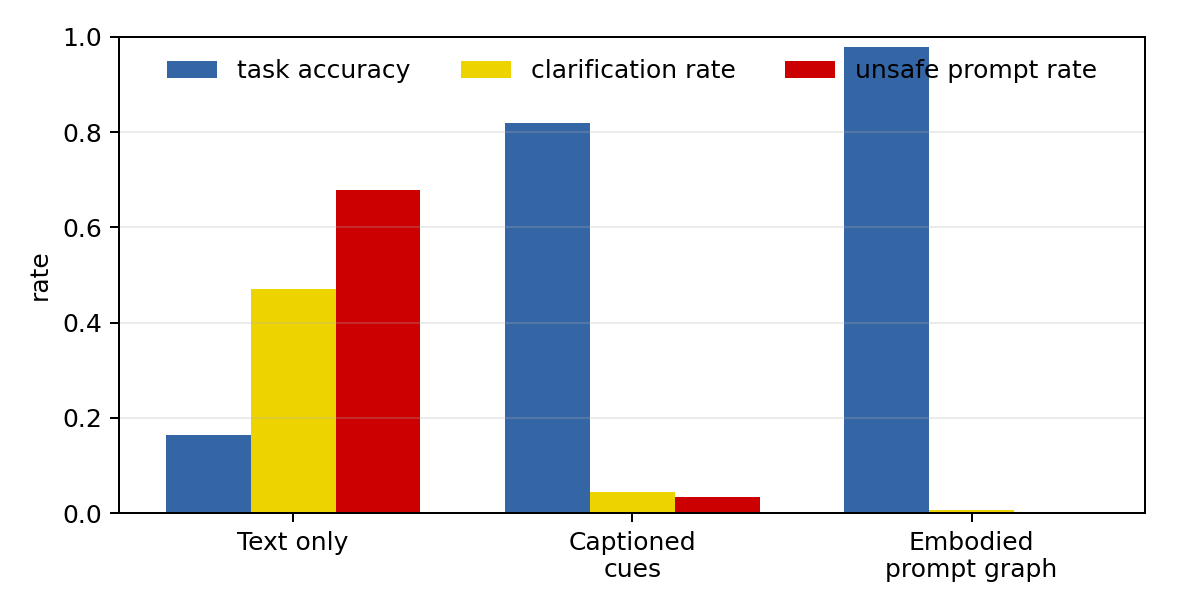
\includegraphics[width=0.82\linewidth]{figures/nonverbal_prompt_metrics.png}}{\fbox{\parbox{0.78\linewidth}{Metric figure unavailable.}}}
\caption{Encoding nonverbal prompts as physical state improves action selection while reducing unsafe execution.}
\label{fig:metrics}
\end{figure}

Table~\ref{tab:diagnostic} and Figure~\ref{fig:metrics} show the intended behavior. Text-only prompting often guesses when the text channel is absent or generic. Captioned cues improve action choice, but still fail when an isolated cue conflicts with object affordance. The embodied prompt graph keeps cue geometry and affordance together, so it can treat open palms and fixture taps as action boundaries rather than optional descriptive tokens.

Table~\ref{tab:v2-binding} stress-tests the safety premise. We keep the original cases and predictions, but on a fraction of safety-critical examples the graph misses the physical safety binding and falls back to the text-only channel. A 2\% binding-miss rate already creates 4 unsafe executions out of 180 safety cases. A 5\% miss rate creates 8 unsafe executions and an unsafe rate of 0.044, worse than the captioned-cue unsafe rate of 0.033. At 20\% binding misses, unsafe execution rises to 0.189. The graph representation is therefore useful only if safety cues are bound conservatively enough to trigger halts or clarification.

\section{Limitations}

This is a synthetic diagnostic benchmark. It does not prove cross-cultural gesture interpretation, perception robustness, or hardware safety. The mechanism also assumes reliable cue detection and object binding. The v2 stress makes that assumption central: missed safety bindings can make the graph less safe than a captioned-cue baseline. Those assumptions are deliberately exposed: if perception cannot bind the cue, the graph should ask for clarification or halt rather than fall back to text-only intent.

\section{Conclusion}

Nonverbal prompts are not second-class language. They are physical task variables. Representing them as an embodied prompt graph gives robot instruction following a clearer contract: act when cue, object, affordance, and safety state agree; clarify when they do not.

\begin{thebibliography}{9}
\bibitem[Argall et~al.(2009)Argall, Chernova, Veloso, and Browning]{argall2009}
Brenna D. Argall, Sonia Chernova, Manuela Veloso, and Brett Browning.
\newblock A survey of robot learning from demonstration.
\newblock \emph{Robotics and Autonomous Systems}, 2009.

\bibitem[Tellex et~al.(2011)Tellex, Kollar, Dickerson, Walter, Banerjee, Teller, and Roy]{tellex2011}
Stefanie Tellex, Thomas Kollar, Steven Dickerson, Matthew R. Walter, Ashis G. Banerjee, Seth Teller, and Nicholas Roy.
\newblock Understanding natural language commands for robotic navigation and mobile manipulation.
\newblock In \emph{AAAI}, 2011.

\bibitem[Cakmak and Thomaz(2012)]{cakmak2012}
Maya Cakmak and Andrea L. Thomaz.
\newblock Designing robot learners that ask good questions.
\newblock In \emph{HRI}, 2012.

\bibitem[Ahn et~al.(2022)]{ahn2022}
Michael Ahn et~al.
\newblock Do as I can, not as I say: Grounding language in robotic affordances.
\newblock In \emph{Conference on Robot Learning}, 2022.

\bibitem[Brohan et~al.(2023)]{brohan2023}
Anthony Brohan et~al.
\newblock RT-1: Robotics transformer for real-world control at scale.
\newblock In \emph{Robotics: Science and Systems}, 2023.

\bibitem[Driess et~al.(2023)]{driess2023}
Danny Driess et~al.
\newblock PaLM-E: An embodied multimodal language model.
\newblock In \emph{International Conference on Machine Learning}, 2023.

\bibitem[Jiang et~al.(2023)]{jiang2023}
Yunfan Jiang et~al.
\newblock VIMA: General robot manipulation with multimodal prompts.
\newblock In \emph{International Conference on Machine Learning}, 2023.

\bibitem[Chi et~al.(2023)]{chi2023}
Cheng Chi et~al.
\newblock Diffusion policy: Visuomotor policy learning via action diffusion.
\newblock In \emph{Robotics: Science and Systems}, 2023.
\end{thebibliography}

\end{document}
